\documentclass[12pt]{beamer}
\usetheme{Warsaw}
\usepackage[utf8]{inputenc}
\usepackage[spanish]{babel}
\usepackage{amsmath}
\usepackage{amsfonts}
\usepackage{amssymb}
\usepackage{graphicx}
\usepackage{color}
\definecolor{softgray}{rgb}{0.8,0.8,0.8}
\usepackage{listings} %Para codigo
\author{Daniel Bolaños Martínez, José María Borrás Serrano, Santiago De Diego De Diego, Fernando De la Hoz Moreno}
\title{Práctica 2: Algoritmos Divide y Vencerás}
\setbeamercovered{transparent} 
\setbeamertemplate{navigation symbols}{} 
%\logo{} 
\institute{ETSIIT} 
\date{} 

%\subject{} 
\begin{document}

\begin{frame}
\titlepage
\end{frame}

\begin{frame}{Introducción}
Nos ha tocado resolver el ejercicio serie unimodal de números.

\vspace{5mm} %5mm vertical space

Para ello, hemos diseñado un algoritmo basado en “divide y vencerás” el cual tiene como objetivo encontrar el valor máximo de una serie unimodal. El orden de eficiencia de este algoritmo es $O(log(n))$ y lo hemos comparado con el algoritmo trivial para este problema que es de orden $O(n)$.
\end{frame}
\begin{frame}{Desarrollo de la Práctica}
Para la comparación hemos obtenido unas tablas en las que se muestran el tiempo de ejecución según distintos número de elementos en los vectores, hemos representado los datos en una gráfica y hemos ajustado estos datos a la función obtenida por la eficiencia teórica por el ajuste de mínimos cuadrados.
\end{frame}

\begin{frame}[fragile]{Código Divide y Vencerás}
	\lstset{language=C++, breaklines=true, extendedchars=true,backgroundcolor=\color{softgray}, keywordstyle=\color{blue},stringstyle=\color{orange},caption={Función unimodal DyV}, basicstyle=\tiny}
	\begin{lstlisting}
int unimodal(vector<int> v)
{
	bool fin=false;
	int maximo=v.size()-1;
	int indice=maximo/2;
	int minimo;
 
	while(!fin)
	{
        if(v.at(indice-1)<v.at(indice))
           if(v.at(indice+1)<v.at(indice))
			    fin=true;
		   else
		   {
				minimo=indice;
				indice=indice+((maximo-indice)/2);
			}
		else
		{
			maximo=indice;
			indice=minimo+((indice-minimo)/2);
		}
	}
	return indice;
}
	\end{lstlisting}
\end{frame}
\begin{frame}[fragile]
	\lstset{language=C++, breaklines=true, extendedchars=true, caption={Función main DyV},backgroundcolor=\color{softgray},keywordstyle=\color{blue},stringstyle=\color{orange},basicstyle=\tiny}
	\begin{lstlisting}
int main(int argc, char* argv[])
{
	vector<int> array;
  	int valor = -1;
	double suma=0;

	int v_size = atoi(argv[1]);
	array.resize(v_size);

	for(int i=0; i<100; ++i)
	{
		int p = 1 + rand() % (v_size-2);
  		array.at(p) = v_size-1;
  		for (int i=0; i<p; i++)
  			array.at(i)=i;
  		for (int i=p+1; i<v_size; i++)
  			array.at(i)=v_size-1-i+p;

		clock_t tantes;
		clock_t tdespues;
		tantes=clock();
		valor = unimodal(array);
		tdespues=clock();
		suma += (double)(tdespues - tantes) / CLOCKS_PER_SEC;
	}
  	cout << v_size <<" "<< suma/100 << endl;
}
	\end{lstlisting}

\end{frame}

\begin{frame}[fragile]{Código secuencial}
	\lstset{language=C++, breaklines=true, extendedchars=true,backgroundcolor=\color{softgray}, keywordstyle=\color{blue},stringstyle=\color{orange},caption={Función unimodal Secuencial}, basicstyle=\footnotesize}
	\begin{lstlisting}
int unimodal_secuencial(vector<int> v)
{
	bool fin=false;
  	int indice=1;

  	while(!fin)
  	{
     	if(v.at(indice+1)<v.at(indice))
      		fin=true;
     	else
      		indice++;
  	}

  	return indice;
}
	\end{lstlisting}
\end{frame}

\begin{frame}[fragile]
	\lstset{language=C++, breaklines=true, extendedchars=true, caption={Función main Secuencial},backgroundcolor=\color{softgray},keywordstyle=\color{blue},stringstyle=\color{orange},basicstyle=\tiny}
	\begin{lstlisting}
int main(int argc, char* argv[])
{
	vector<int> array;
  	int valor = -1;
	double suma=0;

  	int v_size = atoi(argv[1]);
  	array.resize(v_size);

	for(int i=0; i<100; ++i)
	{
		int p = 1 + rand() % (v_size-2);
  		array.at(p) = v_size-1;
  		for (int i=0; i<p; i++)
  			array.at(i)=i;
  		for (int i=p+1; i<v_size; i++)
  			array.at(i)=v_size-1-i+p;

  		clock_t tantes;
  		clock_t tdespues;
  		tantes=clock();
  		valor = unimodal_secuencial(array);
  		tdespues=clock();
		suma += (double)(tdespues - tantes) / CLOCKS_PER_SEC;
	}
  	cout << v_size <<" "<< suma/100 << endl;
}
	\end{lstlisting}

\end{frame}

\begin{frame}{Tabla Datos}


\end{frame}

\begin{frame}{Eficiencia en el caso secuencial}

\begin{figure}[H] 
\centering
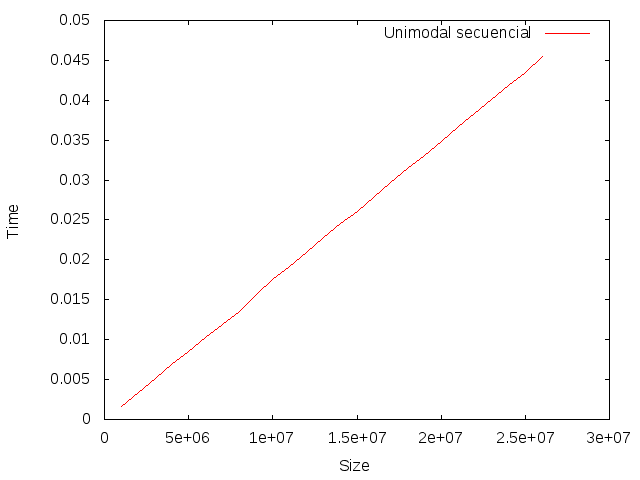
\includegraphics[angle=0,scale=0.5]{img/Eficiencia_sec.png} 
\end{figure}

\end{frame}

\begin{frame}{Eficiencia en el caso Divide y Vencerás}

\begin{figure}[H] 
\centering
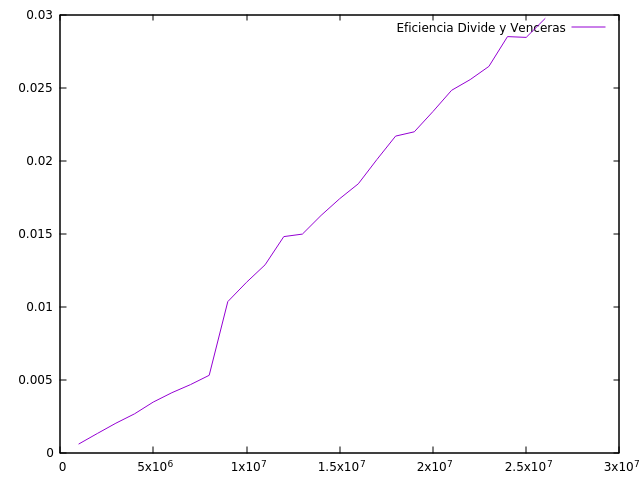
\includegraphics[angle=0,scale=0.5]{img/Eficiencia_dyv.png} 
\end{figure}

\end{frame}

\begin{frame}{Ajuste híbrido en el caso secuencial}

\begin{figure}[H] 
\centering
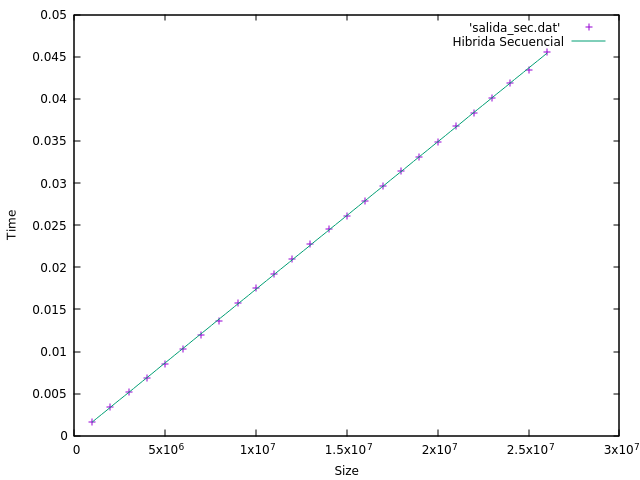
\includegraphics[angle=0,scale=0.5]{img/AjusteHibridoSec.png} 
\caption{Ajustada a la función $f(x)=a_0*x+a_1$} 
\end{figure}

\end{frame}

\begin{frame}
\[
f(x)=a_0*x+a_1 
\]
\[
a_0=1.69539e-09
\]
\[
a_1=-0.00183396
\]
\end{frame}

\begin{frame}{Ajuste híbrido en el caso Divide y Vencerás}

\begin{figure}[H] 
\centering
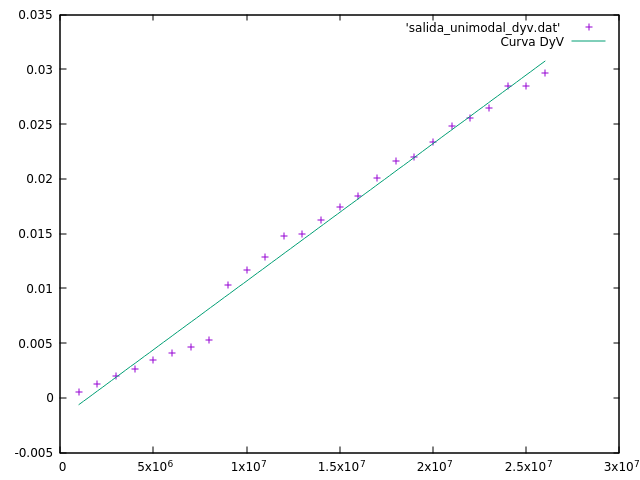
\includegraphics[angle=0,scale=0.5]{img/AjusteHibridoDyV.png} 
\caption{Ajustada a la función $f(x)=a_0*log(x)+a_1*x+a_2$} 
\end{figure}

\end{frame}

\begin{frame}
\[
f(x)=a_0*log(x)+a_1*x+a_2
\]
\[
a_0=1.69539e-09
\]
\[
a_1=1.25523e-09
\]
\[
a_2=-0.00189877
\]
\end{frame}

\begin{frame}{Conclusión}
Como hemos podido observar, los algoritmos de Divide y Vencerás son mucho más eficientes y rápidos que los que podamos pensar de primeras para dar solución a un problema, esto básicamente funciona así gracias a la genial idea del método. 

\vspace{5mm} %5mm vertical space

Dividiendo el problema en otros más pequeños y descartando las soluciones que no sean adecuadas, consiguiendo mayor eficiencia y rapidez que realizando un algoritmo de forma Greedy o de la primera forma que se nos ocurriese.
\end{frame}

\end{document}
\grid
